\documentclass[10pt,a4paper]{amsart}
\usepackage[margin=19mm]{geometry}
\usepackage{amsmath,amssymb,mathtools}
\usepackage[scr=rsfs,cal=euler]{mathalfa}
\usepackage{xfrac}
\usepackage[unicode,hidelinks,bookmarks=false]{hyperref}
\newcommand{\ie}{i.e.\ }
\newcommand{\cf}{cf.\ }
\newcommand{\resp}{respectively\ }
\newcommand{\Subsection}{\subsection}
\providecommand{\nobreakdash}{\nobreak\hbox{-}}
\setlength{\emergencystretch}{2em}
\multlinegap0pt
\usepackage{tikz}
\usepackage{amssymb}
\usepackage{xcolor}
\newtheorem{assumption}{Assumption}
\newtheorem{lemma}{Lemma}
\newtheorem{proposition}{Proposition}
\newcommand{\dsigma}{\mathrm{d}\sigma}
\newcommand{\dt}{\mathrm{d}t}
\newcommand{\dx}{\mathrm{d}x}
\title{A \texorpdfstring{$\varphi$}{phi}-FEM approach for time-dependent domains with unfitted meshes}
\author{Michel Duprez, Johan Marguet, Alexei Lozinski, Igor Voulis}
\date{Source: arXiv:2609.15630v1 (CC BY 4.0)}
\begin{document}
\maketitle

\noindent\emph{Source and licence.} A \texorpdfstring{$\varphi$}{phi}-FEM approach for time-dependent domains with unfitted meshes. Version arXiv:2609.15630v1 (CC BY 4.0), distributed by arXiv under the Creative Commons Attribution 4.0 International licence, http://creativecommons.org/licenses/by/4.0/, as recorded in the arXiv licence metadata for this exact version and shown on the abstract page https://arxiv.org/abs/2609.15630v1. Full licence notice: \texttt{licenses/arxiv-2609.15630-CC-BY-4.0.txt}.\par\smallskip

\noindent\textit{Editorial scope.} Counted unit: the article's proposition coerc (source0.tex lines 915--929). The article's complete original proof of it is delivered with it (source0.tex lines 931--957, one \texttt{proof} environment of 27 lines). No mathematics is written, repaired or re-derived: the statement and the proof are the article's own lines, in the article's own notation, and no retained line is substituted or re-flowed.  Retained uncounted as the source-local context the proof needs: lines 405--416; lines 424--432; lines 440--487; lines 635--638; lines 682--707; lines 762--770; lines 782--788; lines 808--820.  Nothing was omitted from any retained span, so the package carries no omission record.  No retained line contains a citation, so the wrapper carries no bibliography and no bibliography entry.  The retained lines contain the article's own diagram code, which the wrapper typesets with the standard tikz packages; no image file is delivered and the package declares no asset dependency.  Editorial formatting only, in addition: an AMS \texttt{amsart} preamble that restates the article's own declarations and macros used by the retained lines, namely the environments \texttt{assumption}, \texttt{lemma}, \texttt{proposition} on separate counters, together with the standard packages those lines need.  The retained environments print in this document as Assumption 1, Lemma 1, Proposition 1 in order of appearance, whereas the article prints the same items with the numbering of its own full document.  The complete native source of the article as distributed in the arXiv e-print for this exact version is bundled unchanged as \texttt{sources/210434/source0.tex}.
\begin{assumption}\label{asm0}
	At any time $t\in[0,T]$, the boundary $\Gamma(t)$ can be covered by open sets $\mathcal{U}_i$, $i=1,\ldots,N_{\mathcal{U}}=N_{\mathcal{U}}(t)$, and one can introduce on every $\mathcal{U}_i$ local coordinates $\xi_1,\ldots,\xi_d$ with $\xi_d=\varphi(t,\cdot)$ such that all the partial derivatives $\partial^\alpha\xi/\partial x^\alpha$ and $\partial^\alpha x/\partial \xi^\alpha$ up to order $k+1$ are bounded by some $C_{\xi}>0$, uniformly in $t$ and $i$. 
	{Moreover, there exist a positive integer $N_\text{over}$ and $\delta,m>0$, all independent of $t$ and $i$, such that
	\begin{itemize}
		\item[(i)] in the local coordinates $\xi_1,\ldots,\xi_d$ on $\mathcal{U}_i$, this set is a cylinder $\omega_i\times(-\delta,\delta)$;  %in particular, any point of $\mathcal{U}_i$ is connected to $\Gamma(t)$ by the coordinate segment $\xi_1,\ldots,\xi_{d-1}=\mathrm{const}$ lying inside $\mathcal{U}_i$;
		\item[(ii)] %any point of $\mathcal{O}$ belongs to at most $N_0$ sets $\mathcal{U}_i$, and 
		%there exists a partition of unity $\{\chi_i\}$ subordinate to the covering $\{\mathcal{U}_i\}$ such that $\|\nabla\chi_i\|_{\infty}\leqslant C_\xi$, uniformly in $t$ and $i$;
		each $\mathcal{U}_i$ has a non-empty intersection with at most $N_\text{over}-1$ other $\mathcal{U}_j$, $j\not =i$;
		\item[(iii)] $|\varphi(t,\cdot)|\ge m$ on $\mathcal{O}\setminus\cup_{i=1,\ldots,N_{\mathcal{U}}}\mathcal{U}_i$ with some $m>0$;
		\item[(iv)] for every $n=1,\ldots,N$ and every $t\in I_n$,  $\Omega_h^{n,\Gamma}\subset\cup_{i=1,\ldots,N_{\mathcal{U}}}\mathcal{U}_i$.   
	\end{itemize}}
\end{assumption}

\begin{assumption}\label{asm2}
	For every $n\in\{1,\ldots,N\}$, the cells of the boundary submesh $\mathcal{T}_h^{n,\Gamma}$ can be {distributed among} patches $\{\Pi_i \}_{i = 1,\ldots, N_{\Pi}}$, {each patch being made of some cells of $\mathcal{T}_h^{n,\Gamma}$ together with one additional cell taken in the interior,} having the following properties (cf. Fig. \ref{FigPatch}):
	\begin{itemize}
		\item Each patch $\Pi_i$ is a connected set composed of a mesh cell $T_i\in\mathcal{T}_h^n\setminus\mathcal{T}_h^{n,\Gamma}$ and some mesh elements in $\mathcal{T}_h^{n,\Gamma}$. More precisely, $\Pi_i = \{T_i\} \cup \Pi_i^{\Gamma}$ with $\Pi_i^{\Gamma}{}\subset\mathcal{T}_h^{n,\Gamma}$ containing at most $M_\Pi$ cells;
		\item $\mathcal{T}_h^{n,\Gamma} = \cup_{i = 1}^{N_{\Pi}} \Pi_i^{\Gamma}$;
		\item $\Pi_i \cap \Pi_j = \varnothing$ if $i \neq j$.
	\end{itemize}
	By a slight abuse of notation, we shall also write $\Pi_i$ and $\Pi_i^\Gamma$ for the corresponding open domains, i.e. the interiors of $\cup_{T\in\Pi_i}T$ and of $\cup_{T\in\Pi_i^\Gamma}T$. The domains $\Pi_i$ are connected.
\end{assumption}

\begin{figure}[tbp]
\centering
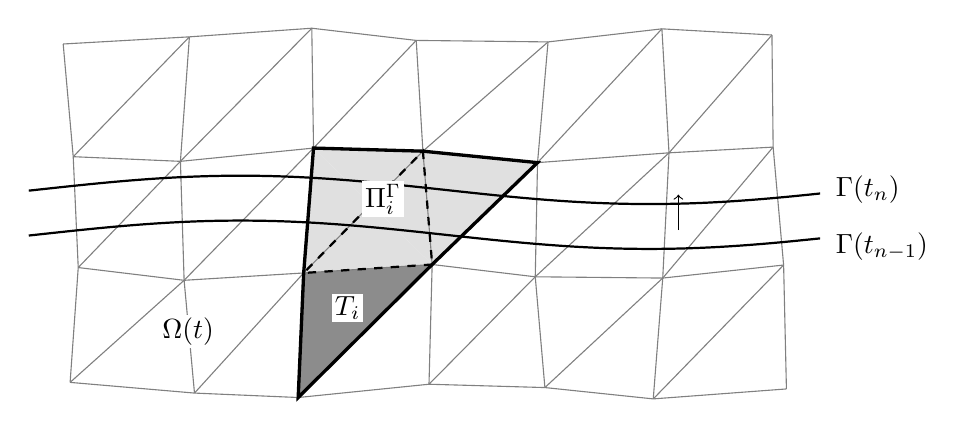
\begin{tikzpicture}[scale=1.5]
	% --- vertices of a slightly perturbed structured mesh ---
	\foreach \i in {0,...,6}{
		\foreach \j in {0,...,3}{
			\pgfmathsetmacro{\xx}{\i+0.07*sin(131*\i+79*\j)}
			\pgfmathsetmacro{\yy}{\j+0.07*cos(107*\i+53*\j)}
			\coordinate (P\i-\j) at (\xx,\yy);
		}
	}
	% --- the cells of the patch ---
	\fill[black!12] (P2-1)--(P3-1)--(P2-2)--cycle;
	\fill[black!12] (P3-1)--(P3-2)--(P2-2)--cycle;
	%\fill[black!12] (P3-1)--(P4-1)--(P4-2)--cycle;
	\fill[black!12] (P3-1)--(P4-2)--(P3-2)--cycle;
	\fill[black!45] (P2-0)--(P3-1)--(P2-1)--cycle;
	% --- the background mesh ---
	\foreach \i/\ii in {0/1,1/2,2/3,3/4,4/5,5/6}{
		\foreach \j in {0,...,3}{ \draw[gray,thin] (P\i-\j)--(P\ii-\j); }
	}
	\foreach \i in {0,...,6}{
		\foreach \j/\jj in {0/1,1/2,2/3}{ \draw[gray,thin] (P\i-\j)--(P\i-\jj); }
	}
	\foreach \i/\ii in {0/1,1/2,2/3,3/4,4/5,5/6}{
		\foreach \j/\jj in {0/1,1/2,2/3}{ \draw[gray,thin] (P\i-\j)--(P\ii-\jj); }
	}
	% --- the patch: outer boundary and interior faces ---
	\draw[very thick] (P2-0)--(P3-1)--(P4-2)--(P3-2)--(P2-2)--(P2-1)--cycle;
	\draw[thick,dashed] (P3-1)--(P2-1)--(P3-2)--cycle;
	%\draw[thick,dashed] (P3-1)--(P2-1);
	%\draw[thick,dashed] (P2-1)--(P3-2);
	%\draw[thick,dashed] (P3-1)--(P3-2);
	% --- the moving boundary ---
	\draw[thick,smooth,variable=\x,domain=-0.35:6.35,samples=80]
	     plot ({\x},{1.32+0.12*sin(52*\x+15)});
	\draw[thick,smooth,variable=\x,domain=-0.35:6.35,samples=80]
	     plot ({\x},{1.70+0.12*sin(52*\x+15)});
	\draw[->] (5.15,1.36)--(5.15,1.66);
	\node[anchor=west] at (6.4,1.22) {$\Gamma(t_{n-1})$};
	\node[anchor=west] at (6.4,1.70) {$\Gamma(t_n)$};
	\node[fill=white,inner sep=1pt] at (1.0,0.5) {$\Omega(t)$};
	% --- labels ---
	\node[fill=white,inner sep=1pt] at (2.65,1.62) {$\Pi_i^\Gamma$};
	\node[fill=white,inner sep=1pt] at (2.35,0.70) {$T_i$};
\end{tikzpicture}
\caption{A sketch of a patch $\Pi_i$ from Assumption \ref{asm2}, in the situation where the boundary moves from $\Gamma(t_{n-1})$ to $\Gamma(t_n)$ during the time slab $I_n$. Light grey: the cells of $\Pi_i^\Gamma \subset \mathcal{T}_h^{n,\Gamma}$, i.e. cells visited by the boundary during $I_n$; dark grey: the cell $T_i\in\mathcal{T}_h^n\setminus\mathcal{T}_h^{n,\Gamma}$, so that $T_i\subset\Omega(t)$ for every $t\in I_n$; and so $\Pi_i = \{T_i\} \cup \Pi_i^\Gamma$. The dashed segments are the interior faces $\mathcal{F}_i$ of the patch, cf. the proof of Lemma \ref{LemMag1}.}\label{FigPatch}
\end{figure}

\begin{equation}
  \label{3termsIOS} a_h (U_h, U_h) = a_h^{\text{in}} (U_h, U_h) +
  a_h^{\text{out}} (U_h, U_h) + a_h^{\text{stab}} (U_h, U_h) .
\end{equation}

\begin{align}
  \label{BIGbound} a_h^{\text{in}} (U_h, U_h) & + a_h^{\text{out}} (U_h, U_h)
   \geqslant \frac{1}{2}  \int_{\Omega (t_N)} \varphi^2 (t_N) | \tilde{u}_h^N |^2
  \dx + \frac{1}{2}  \int_{\Omega_h^0} \varphi^2 (t_0) | \tilde{u}_h^1 |^2
  \dx
\\
 & + \sum_{n = 1}^N \underbrace{\int_{I_n} \int_{\Omega (t)} | \nabla u^n_h
   |^2 \dx \dt}_{\text{cf. Lemma } \ref{LemMag1}} +
   \sum_{n = 2}^N \frac{1}{2}  \int_{\Omega (t_{n - 1})} \varphi^2 (t_{n - 1})  |
   \tilde{u}_h^n - \tilde{u}_h^{n - 1} |^2 \dx
 \notag   \\
 & - \sum_{n = 1}^N \left[ \frac{h^2}{2 \varepsilon}  \underbrace{\sum_{T\in\mathcal{T}_h^{n,\Gamma}}\int_{I_n}
   \int_{T} \left| \frac{\partial \varphi}{\partial t}
   \tilde{u}_h^n - \Delta u^n_h \right|^2 \dx \dt}_{\text{ part of stabilization}} + \frac{\varepsilon}{2 h^2}
   \underbrace{\sum_{T\in\mathcal{T}_h^{n,\Gamma}}\int_{I_n} \int_{T} |u^n_h |^2 \dx
   \dt}_{\text{ cf.  Lemma } \ref{LemInverse}} \right]
 \notag \\
 & - \sum_{n = 1}^N \left[ \frac{h}{2 \varepsilon}  \underbrace{
  \sum_{F\in\mathcal{F}_h^{n, \Gamma}} \int_{I_n} \int_{F} [\![\partial_\nu u^n_h]\!]^2 \dsigma \dt}_{\text{ part of stabilization}} +
   \frac{\varepsilon}{2 h} \underbrace{ \sum_{F\in\mathcal{F}_h^{n, \Gamma}}\int_{I_n}   \int_{F}|u^n_h |^2 \dsigma \dt}_{\text{cf. Lemma }
   \ref{LemInverse}}  \right]
  \notag \\
    &+ \sum_{n = 2}^N \left[ \frac{1}{2}  \int_{\Omega^n_h \cap B^{n - 1} (t_{n - 1})} \varphi^2 (t_{n - 1}) | \tilde{u}_h^n |^2 \dx \right.
   \left. - \frac{1}{2}  \underbrace{\int_{\Omega^n_h \cap B^{n - 1}  (t_{n - 1})} \varphi^2 (t_{n - 1}) | \tilde{u}_h^{n - 1} |^2 \dx }_{\text{cf. Lemma } \ref{LemInverseT}} \right].
\notag
\end{align}

\begin{lemma}
  \label{LemInverse}Under Assumptions {\ref{asm0}--\ref{asm2}}, there exists $C>0$ such that, for each $n=1,\ldots,N$, {all $h\leqslant h_0$} and $v_h \in  V_h^n$,
  \begin{equation}
    \frac{1}{h^2}  \sum_{T\in\mathcal{T}_h^{n,\Gamma}}\int_{I_n} \int_{T} | \varphi v_h |^2
    \dx \dt + \frac{1}{h} \sum_{F\in\mathcal{F}_h^{n, \Gamma}}   \int_{I_n} \int_{F} | \varphi v_h |^2 \dsigma \dt \leqslant C \int_{I_n}
    \int_{\Omega^n_h} | \nabla (\varphi v_h) |^2 \dx \dt.
    \label{evident1}
  \end{equation}
\end{lemma}

\begin{lemma}
  \label{LemInverseT}Under Assumptions {\ref{asm0}--\ref{asm2}}, there exists $C>0$ such that, for each $n=1,\ldots,N$, {and all $v_h \in  V_h^n$,  $s\in[t_{n-1},t_n]$,}
\begin{equation}
    {\int_{\Omega_h^{n,\Gamma}}} \varphi^2 (s) |v_h |^2 \dx
    \leqslant C {\left(\frac{h^2}{\tau}+\tau\right)}  \int_{I_n} \int_{\Omega^n_h} | \nabla (\varphi v_h) |^2 \dx \dt \,. \label{evident2}
  \end{equation}
\end{lemma}

\begin{lemma}
	\label{LemMag1}
	Under Assumptions~\ref{asm0}--\ref{asm2}, there exist constants $C,h_0>0$, depending only on the regularity of the mesh $\mathcal{T}_h^{\mathcal{O}}$, on $k$ and on the constants of Assumptions~\ref{asm0}--\ref{asm2}, such that for all $h\leqslant h_0$, all $n=1,\ldots,N$ and all $v_h \in V_h^n$,
	\begin{multline*}
		\int_{I_n} \int_{\Omega_h^n} | \nabla (\varphi v_h) |^2 \, \dx \, \dt
		\leq C \Bigg(
		\int_{I_n} \int_{\Omega(t)} | \nabla (\varphi v_h) |^2 \, \dx \, \dt \\
		+ h^2 \sum_{T\in\mathcal{T}_h^{n,\Gamma}}\int_{I_n} \int_{T}
		\left| \frac{\partial \varphi}{\partial t} v_h - \Delta (\varphi v_h) \right|^2 \, \dx \, \dt
		+ h \sum_{F\in\mathcal{F}_h^{n, \Gamma}} \int_{I_n}  \int_{F}	 [\![\partial_\nu (\varphi v_h)]\!] ^2 \, \dsigma \, \dt
		\Bigg).
	\end{multline*}
\end{lemma}

\begin{proposition}\label{coerc}
Assuming $\gamma$ big enough, $h\leqslant h_0$ and $\frac{h^2}{\tau}+\tau$ small  enough, it holds for any $U_h\in\mathbb{V}_h$
  \begin{multline*}
       a_h (U_h, U_h) \geqslant \frac{1}{2}  \int_{\Omega (t_N)} \varphi^2 (t_N) |
     \tilde{u}_h^N |^2 \dx + \frac{1}{2}  \int_{\Omega_h^0} \varphi^2 (t_0)
     | \tilde{u}_h^1 |^2 \dx \\
   + c \sum_{n = 1}^N \int_{I_n} \int_{\Omega^n_h} | \nabla u^n_h |^2 \dx \dt + \frac{1}{2} \sum_{n = 2}^N  \int_{\Omega (t_{n - 1})} \varphi^2
     (t_{n - 1})  | \tilde{u}_h^n - \tilde{u}_h^{n - 1} |^2 \dx \\
   + \frac{1}{2} \sum_{n = 1}^N \left[ \ \gamma h
   \sum_{F\in\mathcal{F}_h^{n, \Gamma}}  \int_{I_n}\int_{F}[\![\partial_\nu u^n_h]\!]^2 \dsigma \dt + \gamma h^2 \sum_{T\in\mathcal{T}_h^{n,\Gamma}} \int_{I_n} \int_{T}
     \left| \frac{\partial \varphi}{\partial t}  \tilde{u}^n_h - \Delta u^n_h
     \right|^2 \dx \dt \right]
  \end{multline*}
  with a constant $c > 0$.
\end{proposition}

\begin{proof}
  Recall from (\ref{3termsIOS}) that $a_h (U_h, U_h)$ is the sum of three
  contributions ``in'', ``out'', and ``stab'', and that the sum of the contributions ``in''  and ``out'' is bounded from below in (\ref{BIGbound}).
  Let us make precise the order in which the preceding lemmas are applied. %, since the negative terms of (\ref{BIGbound}) are controlled by integrals over $\Omega_h^n$, whereas the only positive gradient term available at this stage is an integral over the smaller domain $\Omega (t)$. 
  Set, for brevity,
  \[ G_n^{\mathrm{in}} = \int_{I_n} \int_{\Omega (t)} | \nabla u^n_h |^2 \dx \dt , \qquad
     G_n = \int_{I_n} \int_{\Omega^n_h} | \nabla u^n_h |^2 \dx \dt , \]
  \[ S_n = h \sum_{F\in\mathcal{F}_h^{n, \Gamma}}\int_{I_n} \int_{F} [\![\partial_\nu u^n_h]\!]^2 \dsigma \dt
     + h^2 \sum_{T\in\mathcal{T}_h^{n,\Gamma}}\int_{I_n} \int_{T} \left| \frac{\partial \varphi}{\partial t}  \tilde{u}_h^n - \Delta u^n_h \right|^2 \dx \dt , \]
  so that $a_h^{\mathrm{stab}}(U_h,U_h)=\gamma\sum_n S_n$ and the two ``parts of stabilization'' underbraced in (\ref{BIGbound}) sum up to $\frac{1}{2\varepsilon}S_n$.
  Lemma \ref{LemInverse} bounds the two underbraced terms of (\ref{BIGbound}) carrying the factor $\varepsilon$ by $c_0\varepsilon\, G_n$. Lemma \ref{LemInverseT}, applied at rank $n-1$ with $s=t_{n-1}$ and $v_h=\tilde u_h^{n-1}$, bounds the last underbraced term by $c_2\left(\frac{h^2}{\tau}+\tau\right) G_{n-1}$; here we have used the inclusion
  \[ \Omega^n_h \cap B^{n - 1} (t_{n - 1}) = \Omega_h^n\cap\big(\Omega_h^{n-1}\setminus\Omega(t_{n-1})\big)
  \subset \Omega_h^{n-1}\setminus\Omega(t_{n-1})
  \subset \Omega_h^{n-1,\Gamma} \,.\]
Lemma \ref{LemMag1} then converts these bounds into
  \[ c_0\varepsilon\, G_n + c_2\left(\frac{h^2}{\tau}+\tau\right) G_{n-1} \leqslant c_1\varepsilon\left(G_n^{\mathrm{in}} + S_n\right) + c_1\left(\frac{h^2}{\tau}+\tau\right)\left(G_{n-1}^{\mathrm{in}} + S_{n-1}\right) . \]
  Reporting this into (\ref{BIGbound}), summing in $n$ and adding the stabilization $a_h^{\mathrm{stab}}(U_h,U_h)$, we arrive at
  \begin{multline*} a_h (U_h, U_h) \geqslant \frac{1}{2}  \int_{\Omega (t_N)} \varphi^2 (t_N) |
	\tilde{u}_h^N |^2 \dx + \frac{1}{2}  \int_{\Omega_h^0} \varphi^2 (t_0) |
	\tilde{u}_h^1 |^2 \dx \\
	+ \sum_{n = 1}^N \left( 1-c_1 \varepsilon - c_1 \left(\frac{h^2}{\tau}+\tau\right) \right) G_n^{\mathrm{in}} +
	\sum_{n = 2}^N \frac{1}{2}  \int_{\Omega (t_{n - 1})} \varphi^2 (t_{n - 1})  |
	\tilde{u}_h^n - \tilde{u}_h^{n - 1} |^2 \dx \\
	+ \sum_{n = 1}^N \left( \gamma -c_1\varepsilon - c_1\left(\frac{h^2}{\tau}+\tau\right) - \frac{1}{2 \varepsilon} \right) S_n .
\end{multline*}
    We now choose $\varepsilon$ small enough and assume $\frac{h^2}{\tau}+\tau$ small enough so that $c_1\varepsilon+c_1\left(\frac{h^2}{\tau}+\tau\right)\leqslant \frac12$, and then $\gamma$ big enough so that $\gamma-c_1\varepsilon-c_1\left(\frac{h^2}{\tau}+\tau\right)-\frac{1}{2\varepsilon}\geqslant \frac{\gamma}{2}+\frac12$. A last application of Lemma \ref{LemMag1}, in the form $G_n \leqslant c_1 (G_n^{\mathrm{in}} + S_n)$, allows us to replace $\frac12 (G_n^{\mathrm{in}} + S_n)$ by $\frac{1}{2c_1} G_n$, which gives the announced coercivity estimate with $c=\frac{1}{2c_1}$, the gradient term being now integrated over the whole of $\Omega_h^n$ and the remaining $\frac{\gamma}{2}S_n$ giving the last line of the statement.
\end{proof}

\end{document}
